\documentclass[compress, darktitle, framenumber, totalframenumber]{beamer}
\usepackage{mathtools}
\usepackage{tikz}
\usepackage{wrapfig}
\usepackage{xparse}

\mathtoolsset{showonlyrefs}

\usetheme{UniversiteitAntwerpen}

\title{Wisku$\mathbb{N}$de in-$\mathbb{Z}$icht}
\subtitle{Wiskunde in muziek}
\author{Pieter Belmans (\texttt{pieter.belmans@uantwerpen.be}) \\ Matthias Roels (\texttt{matthias.roels@uantwerpen.be})}
\date{9 januari 2014}

\begin{document}
\begin{frame}
  \titlepage
\end{frame}

\begin{frame}
  \frametitle{Wie zijn wij?}
\end{frame}

\begin{frame}
  \frametitle{Wat gaan we vandaag doen?}

  \begin{block}{Voormiddag}
    \begin{wrapfigure}{r}{.5\textwidth}
      \centering
      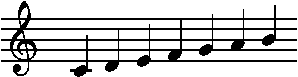
\includegraphics{scores/scale-cropped}
    \end{wrapfigure}
    Waarom do-re-mi-fa-sol-la-si?
    \begin{enumerate}
      \item de structuur van geluid
      \item mooi en lelijk
      \item 7 (of 12) noten
    \end{enumerate}
  \end{block}

  \pause

  \begin{block}{Namiddag}
    Wat maakt geluid muziek?
    \begin{enumerate}
      \item de structuur van geluid analyseren
      \item voorbeelden
      \item verschillen tussen muziekinstrumenten
    \end{enumerate}
  \end{block}
\end{frame}

\begin{frame}
  \frametitle{Vragen staat vrij}
\end{frame}

\section{Wat is geluid?}

\section{Wat zijn boventonen?}
% TODO refer to last part of talk, and afternoon

\section{Hoe maken we verschillende noten?}

\section{Wat klinkt er mooi samen en wat niet?}

\section{Wat is een stemming?}
% TODO: answers the question ``why do we have C D E F G A B''

\section{Wat is het probleem met stemmingen?}

\section{Hoe kunnen we dit oplossen?}

\section{Hoe kan geluid ons bedotten?}
% TODO: end the previous section with a remark hinting at the crappy way we experience sound, ties it in with this last section *and* afternoon
\end{document}

